\documentclass[12pt]{article}
\usepackage[utf8]{inputenc}
\usepackage[brazil]{babel}
\usepackage{amsmath, amssymb, array, bm, geometry, booktabs, siunitx, graphicx, colortbl, parskip, xcolor}
\usepackage{listings}
\usepackage{color}
\usepackage{float}
\usepackage{fancyhdr}
\usepackage{titlesec}
\usepackage{hyperref}
\usepackage{listings}

\setlength{\headheight}{14.5pt}
\addtolength{\topmargin}{-2.5pt}
\geometry{a4paper, total={6in, 9in}}




\definecolor{codegray}{gray}{0.9}
\lstset{
    backgroundcolor=\color{codegray},
    basicstyle=\ttfamily\footnotesize,
    frame=single,
    breaklines=true,
    captionpos=b,
    numbers=left,
    numberstyle=\tiny,
    language=Python
}

% Cabeçalho
\pagestyle{fancy}
\fancyhf{}
\rhead{UnB}
\lhead{Departamento de Ci\^encias Mec\^anicas}
\cfoot{\thepage}

\titleformat{\section}{\large\bfseries}{\thesection}{1em}{}

\begin{document}

% Capa
\begin{titlepage}
    \centering
    
\includegraphics[width=12cm]{img/unb_bandeira.png} \\
    \vspace{1cm}
    \textsc{\Large Universidade de Bras\'ilia} \\
    \textsc{Departamento de Ciências Mec\^anicas} \\
    \textsc{Programa de P\'os-Gradua\c{c}\~ao} \\
    \vfill
    {\Large\bfseries Programa 8} \\
    \vspace{0.5cm}
    {\Large\bfseries Equações Diferenciais} \\
    {\Large\bfseries Tranferência de Calor em Regime Transiente} \\
    {\Large\bfseries Geometria Complexa} \\
    \vspace{0.5cm}
    \textbf{Disciplina: M\'etodos Num\'ericos} \\
    Professor: Dr. Rafael Gabler Gontijo \\
    \vfill
    \textbf{Aluno: Eng. Lucas Wanick — Mestrando em Engenharia Mec\^anica} \\
    \vspace{0.5cm}
        \today \\
\end{titlepage}


\section{Introdução}
O presente relatório documenta o desenvolvimento do último programa do curso de \textit{Métodos Numéricos} ministrado pelo Professor Rafael Gabler Gontijo na Universidade de Brasília.  
O objetivo central foi implementar um solver numérico capaz de resolver a equação de condução de calor estacionária em uma geometria retangular com cantos curvos (adiabáticos), submetida a condições de contorno mistas:

\begin{figure}[H]
    \centering
    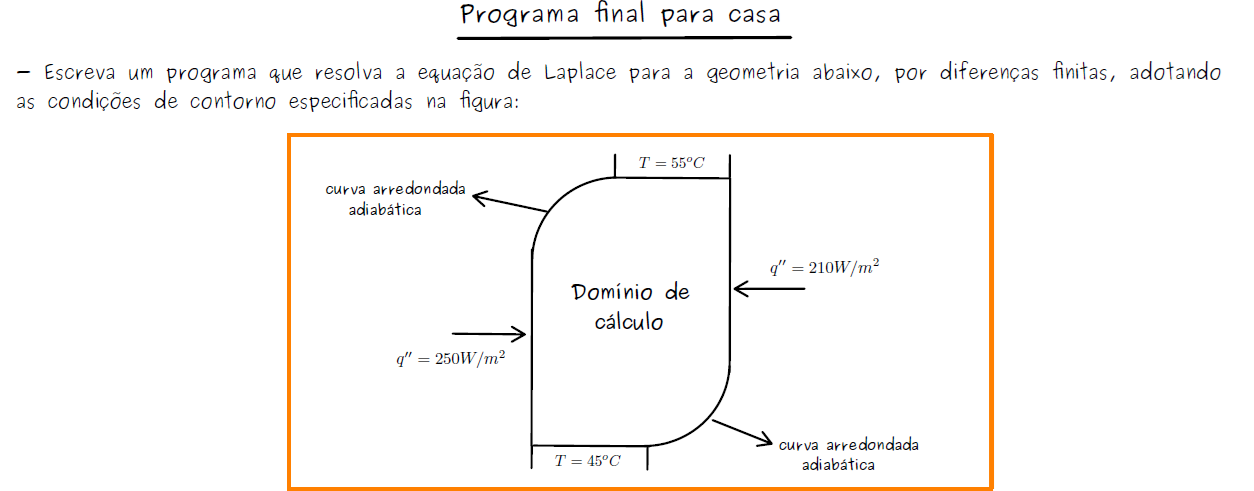
\includegraphics[width=0.8\textwidth]{img/enunciado.png}
    \caption{Enunciado do problema - Lousa da Aula 35.}
\end{figure}

\begin{itemize}
    \item Temperaturas fixas (Dirichlet) nas faces superior e inferior;
    \item Fluxos de calor prescritos (Neumann) nas faces laterais;
    \item Isolamento térmico (condição adiabática) nos cantos arredondados.
\end{itemize}

O desenvolvimento visou obter uma solução robusta, eficiente e escalável, capaz de lidar com malhas refinadas , preservando a fidelidade geométrica e garantindo estabilidade numérica.

\begin{figure}[H]
    \centering
    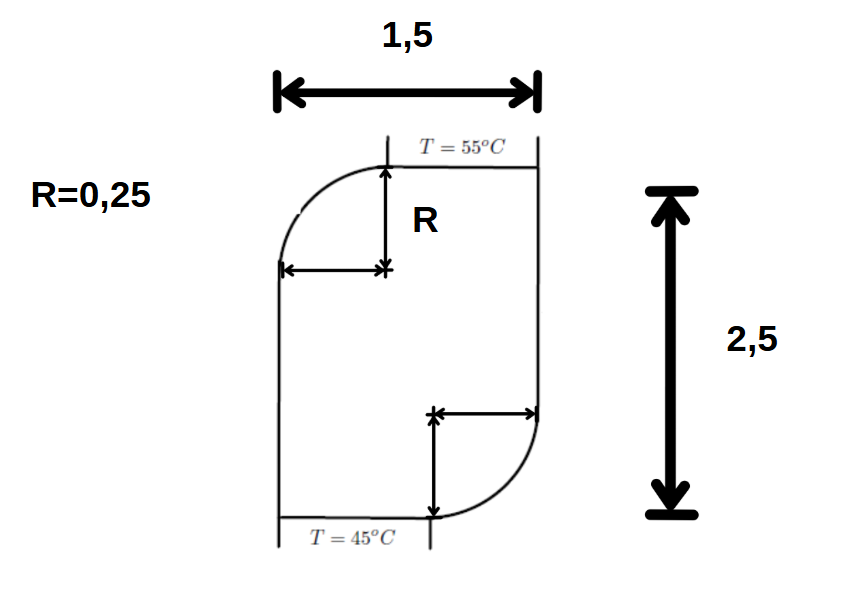
\includegraphics[width=0.6\textwidth]{img/geometria.png}
    \caption{Geometria do problema. Dimenções arbitradas: $L = 1.50\,\mathrm{m}$, $H = 2.50\,\mathrm{m}$, raio dos cantos $R = 0.25\,\mathrm{m}$.}
\end{figure}

\section*{2. Formulação Matemática}

A equação governante é a equação de Laplace bidimensional para regime estacionário ($\nabla^2T=0$):

\begin{equation}
\frac{\partial^2 T}{\partial x^2} + \frac{\partial^2 T}{\partial y^2} = 0
\end{equation}

\subsection*{2.1 Condições de contorno}

\begin{itemize}
    \item \textbf{Dirichlet (superior e inferior):}
    \[
    T(y=0) = 45^\circ C, \qquad T(y=H) = 55^\circ C
    \]
    \item \textbf{Neumann (laterais):}
    \[
    -k \frac{\partial T}{\partial x}\bigg|_{x=0} = q_{\text{left}}, 
    \qquad 
    -k \frac{\partial T}{\partial x}\bigg|_{x=L} = q_{\text{right}}
    \]
    onde $k$ é a condutividade térmica do material, definida como 71 $W/mK$ (Aço) e $q_{left}$, $q_{right}$ são os fluxos de calor prescritos de 250 $W/m^2$ e 210 $W/m^2$, respectivamente.
    \item \textbf{Adiabático (cantos):}
    \[
    \frac{\partial T}{\partial n} = 0
    \]
\end{itemize}

Geometria: $L = 1.50\,\mathrm{m}$, $H = 2.50\,\mathrm{m}$, cantos curvos de raio $R = 0.25\,\mathrm{m}$.

\section*{3. Discretização Numérica}

O domínio foi discretizado em uma malha uniforme de $n \times n$ pontos, utilizando o método das diferenças finitas de 5 pontos:

\begin{equation}
-4T_{i,j} + T_{i+1,j} + T_{i-1,j} + T_{i,j+1} + T_{i,j-1} = 0
\end{equation}

As condições de contorno foram incorporadas da seguinte forma:
\begin{itemize}
    \item \textbf{Dirichlet:} valores fixos diretamente no vetor fonte $b$.
    \item \textbf{Neumann:} usando a formulação ajustada:
    \[
    T_{\text{parede}} = T_{\text{vizinho}} + \frac{q'' \, \Delta x}{k}
    \]
    com compensação na matriz:
    \[
    A_{kk} \leftarrow A_{kk} + 1
    \]
    \item \textbf{Adiabático:} regiões de contorno curvo foram identificadas por verificação geométrica $(x,y)$ e excluídas do sistema.
\end{itemize}

\section*{4. Implementação Computacional}

\begin{itemize}
    \item Linguagem: Python 3.12
    \item Bibliotecas: \texttt{numpy}, \texttt{scipy.sparse} (LIL $\rightarrow$ CSR), \texttt{matplotlib}
\end{itemize}

Estratégias de desempenho:
\begin{itemize}
    \item Matriz esparsa, evitando alocação densa (redução de memória de TB $\rightarrow$ MB).
    \item Solver \texttt{spsolve} para eficiência em sistemas grandes.
    \item Máscaras (\texttt{NaN}) para lidar com cantos adiabáticos.
\end{itemize}

\subsection*{4.1 Geração da malha e classificação dos nós}

A função \texttt{gerar\_malha\_tipo} atribui a cada nó:
\begin{itemize}
    \item \textbf{I:} interno
    \item \textbf{D:} Dirichlet
    \item \textbf{N:} Neumann
    \item \textbf{A:} adiabático
\end{itemize}

\begin{figure}[H]
    \centering
    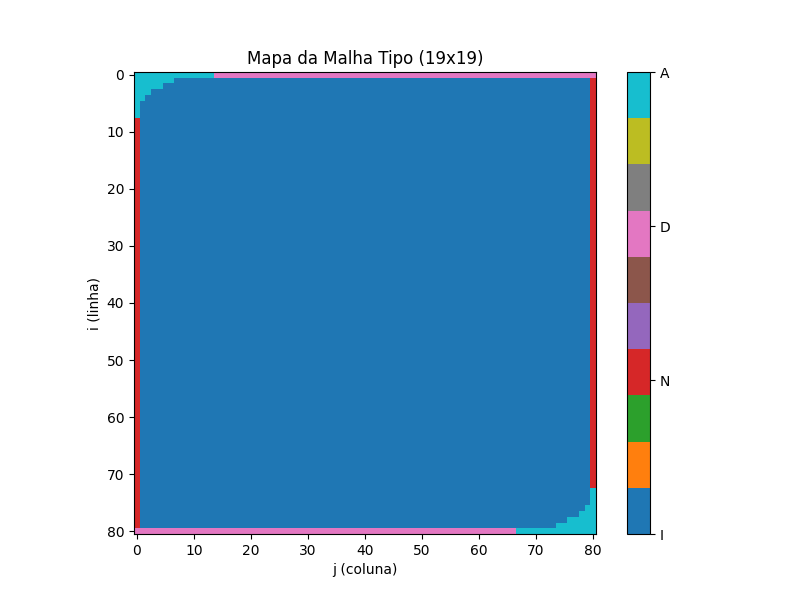
\includegraphics[width=0.8\textwidth]{img/Figure_2.png}
    \caption{Malha gerada com classificação dos nós.}
\end{figure}

\subsection*{4.2 Montagem do sistema}

\begin{itemize}
    \item Mapeamento de incógnitas internas.
    \item Montagem de $A$ e $b$ considerando as diferentes condições.
    \item Implementação rigorosa da Neumann com compensação na diagonal.
\end{itemize}

\subsection*{4.3 Interpolação para visualização}

Pós-processamento para interpolar valores em regiões Neumann e adiabáticas, garantindo visualização contínua sem alterar a solução numérica.

\section*{5. Resultados Numéricos}

\subsection*{5.1 Distribuição de temperatura}

O solver convergiu para distribuições estáveis em malhas de até $729 \times 729$.  
Temperaturas coerentes com as condições impostas:
\begin{itemize}
    \item Regiões centrais mais quentes devido ao aporte de calor lateral.
    \item Gradiente vertical suave entre $45^\circ C$ e $55^\circ C$.
\end{itemize}

\begin{figure}[H]
    \centering
    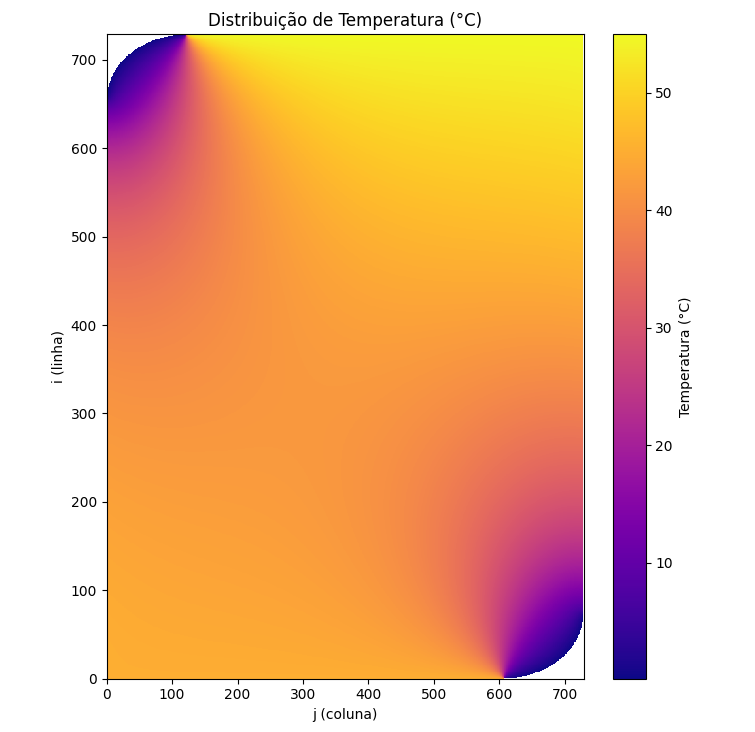
\includegraphics[width=0.8\textwidth]{img/Figure_1.png}
    \caption{Distribuição de temperatura calculada. Valores interpolados para visualização contínua.}
\end{figure}

\subsection*{5.2 Comportamento físico}

\begin{itemize}
    \item Alteração do sinal de $q_{\text{left}}$ ou $q_{\text{right}}$ produz gradientes opostos, confirmando implementação correta da Neumann.
    \item Perfis de fluxo e isolamento térmico nos cantos respeitados.
    \item Balanço energético coerente: fluxo líquido $\rightarrow$ aumento da temperatura média.
\end{itemize}

\section*{6. Conclusão}

O programa desenvolvido cumpre plenamente os objetivos:
\begin{itemize}
    \item Resolver a equação de condução de calor em geometria complexa com múltiplos tipos de contorno.
    \item Suportar malhas muito refinadas com alta eficiência de memória.
    \item Produzir resultados fisicamente coerentes e visualmente interpretáveis.
\end{itemize}

Este projeto encerra o curso com demonstração de proficiência em métodos numéricos, implementação computacional avançada e capacidade analítica de validar soluções numéricas frente à realidade física.

\section*{7. Trabalhos futuros}

\begin{itemize}
    \item Implementação de parâmetros $\alpha$ e $\beta$ para ajuste fino da curvatura em malhas grosseiras.
    \item Extensão para problemas transientes (dependentes do tempo).
    \item Acoplamento com modelos de convecção e radiação para simular trocas térmicas complexas.
\end{itemize}

\end{document}